\section{Desarrollo módulo de análisis de imágenes}

Las imágenes generadas para el conjunto de entrenamiento se formaron insertando los puntos en fondo blanco, teniendo como resultado una imagen binaria (contenido en negro y fondo blanco) por lo que al considerar que las fotogragías tomadas por un dispositivo móvil no iba a generar por sí mismo un formato semejante fue necesario desarrollar un módulo para esta tarea.

\begin{figure}[h]
	\centering
	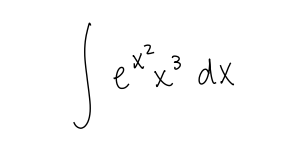
\includegraphics[width=0.4\textwidth]{capitulo5/imageprocessor/example_dataset.png}
	\caption{Imagen de ejemplo del conjunto de entrenamiento generado}
	\label{fig:example_dataset}
\end{figure}

El proceso consiste en convertir el área de la expresión matemática en negro y el resto en fondo blanco, para ello se consideraron las técnicas mencionadas en %ref
 y específicamente se probaron los algoritmos de Otsu y Sauvola \cite{inproceedings}.
 
\begin{figure}[h]
	\centering
	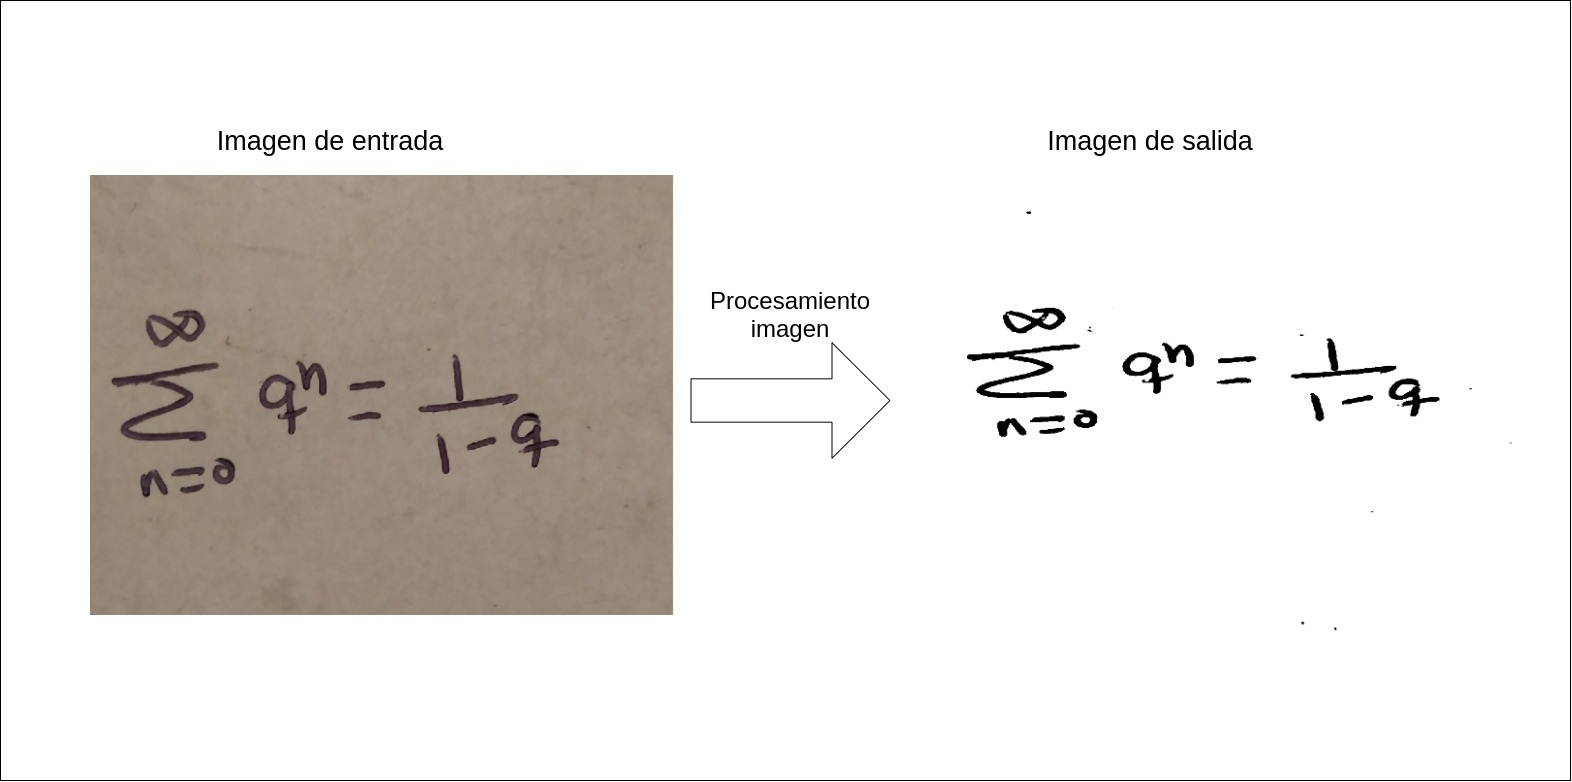
\includegraphics[width=0.8\textwidth]{capitulo5/imageprocessor/IO_image.jpg}
	\caption{Fotografía procesada con algoritmo de Sauvola}
	\label{fig:process_image}
\end{figure}

De acuerdo a lo mencionado en el marco teórico existen técnicas para binarizar una imagen que calculan el umbral de manera automática, dos de estos algoritmos son el algoritmo de Otsu y el algoritmo de Sauvola, a continuación se describen brevemente y se dan detalles de la implementación o uso según el caso.

\subsection{Algoritmo de Otsu}
El método de Otsu evita tener que elegir un valor de umbral y lo determina automáticamente.

Considere una imagen con solos dos valores distintos (imagen bimodal), donde el histograma consistiría solo de dos picos. Un buen valor de umbral sería a la mitad de estos dos valores. Similarmente el método de Otsu determina un valor de umbral óptimo global del histograma de la imagen.

Al tratarse de una imagen bimodal, el algoritmo intenta encontrar un valor de umbral (t) que minimice la varianza ponderada dentro de la clase, dada por la relación:

\begin{equation}
	\sigma _ {w} ^{2}(t) = q_{1}(t) \sigma _{1}^2(t) + q_{2}(t) \sigma _{2}^2(t)
\end{equation}
donde:
\begin{equation}
	\begin{array}{l}
		q_{1}(t) = \sum_{i=1}^{t} P(i) \wedge q_{2}(t) = \sum_{i=t+1}^{I} P(i)\\\\
		\mu_{1}(t) = \sum_{i=1}^{t} \frac{i P(i)}{q_1{t}} \wedge \mu_{2}(t) = \sum_{i=t+1}^{I} \frac{i P(i)}{q_2{t}}\\\\
		\sigma_{1}^2(t) = \sum_{i = 1}^{t} [i - \mu_{1}(t)]^2 \frac{P(i)}{q_{1}(t)} \wedge \sigma_{2}^2(t) = \sum_{i = t+1}^{I} [i - \mu_{2}(t)]^2 \frac{P(i)}{q_{2}(t)}
	\end{array}
\end{equation}

\lstinputlisting[language=Python]{capitulo5/imageprocessor/code_files/otsu.py}

\subsection{Algoritmo de Sauvola}

El algorimo de Sauvola tiene una implementación más extensa por lo que se dispuso de la utilización de la implementación contenida en \textbf{skimage} dentro del paquete filters.
\lstinputlisting[language=Python, firstline=4, lastline=7]{capitulo5/imageprocessor/code_files/scriptCV.py}

\lstinputlisting[language=Python, firstline=26, lastline=30]{capitulo5/imageprocessor/code_files/scriptCV.py}
